\documentclass{beamer}
\usetheme{Frankfurt}

\usepackage{listings}

\newcommand{\todo}[1]{\alert{TODO #1}}

\title{Cryptography}
\subtitle{Lecture 3 \\ Computer Security DD2395}
\author[R. Guanciale]{
  Roberto Guanciale\\
  robertog@kth.se
}
\date{2015-11-05}
\begin{document}

\begin{frame}[plain]
  \titlepage
\end{frame}

\begin{frame}{Outline for Today}
  \begin{itemize}
    \item Cryptographyc Tools
    \item Symmetric encryption
  \end{itemize}
\end{frame}

\begin{frame}{Symmetric encryption}
  \begin{itemize}
  \item Only type of encryption from Julius Caesar until 1970s
  \item Guarantee confidentiality
  \item Guarantee integrity if there is a notion of well-formedness
  \end{itemize}
  \begin{center}
    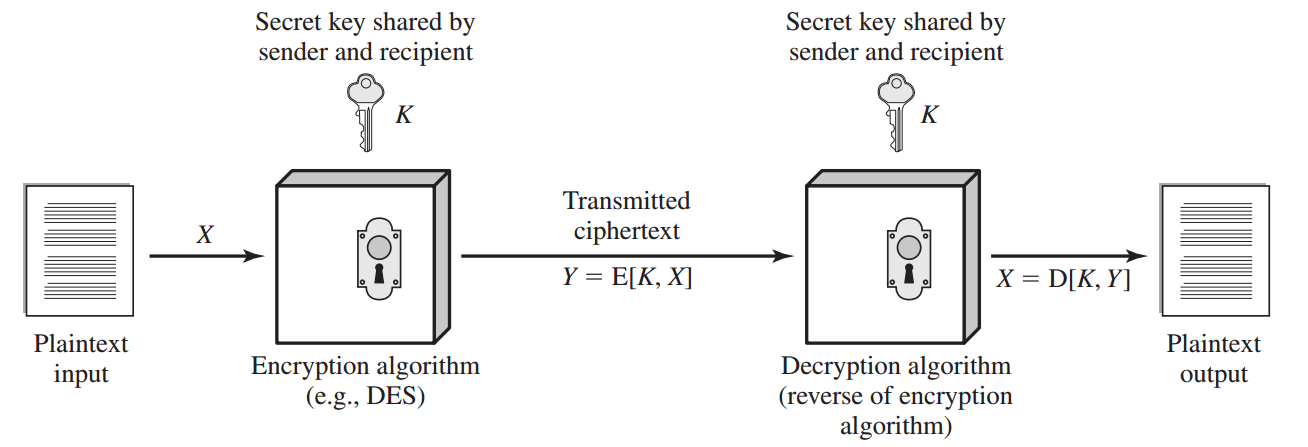
\includegraphics[width=0.9\linewidth]{symm}
  \end{center}
\end{frame}

\begin{frame}{History of cryptography}
  \begin{itemize}
  \item Hieroglyphics 3300 BCE: puzzles
  \item Hebrew scholars and Romans used mono-alphabetic substitution ciphers
  \item Mesopotamia 1500 BCE: clay tablets protecting information about
    recipe for pottery glaze (no open source here)
  \end{itemize}
  
\end{frame}

\begin{frame}{History of cryptography}
  \begin{itemize}
  \item Caesar cipher:
  \begin{itemize}
  \item $K \in [0 \dots 22]$ (23 letters, no U,J and W)
  \item $E_n(m) = (x+K) \ mod\  23$
  \item $D_n(m) = (x-K) \ mod\  23$
  \end{itemize}
\item<2-> Cracked by Al-Kindi, an Arab mathematician, AC 800, using
  crypt-analysis \\
  \begin{center}
    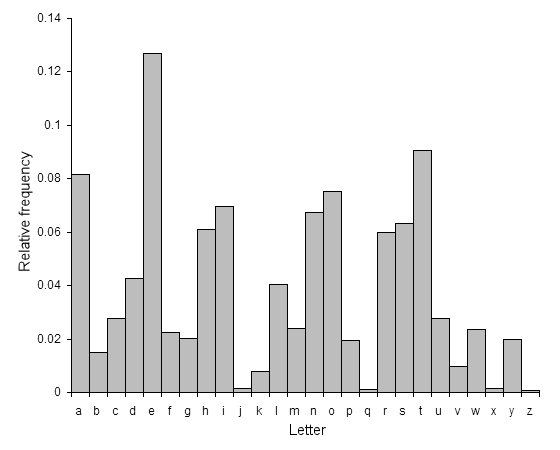
\includegraphics[width=0.4\linewidth]{analysis}
  \end{center}
  \end{itemize}
  
\end{frame}

\begin{frame}{History of cryptography}
  \begin{itemize}
  \item  Leon Battista Alberti around the year AD 1467,
    polyalphabetic cipher, indicating the alphabet change by an
    uppercase letter.
  \item World War II: Enigma vs chess masters and mathematics (Turing)
  \item World War II: Geheimschreiber vs Arne Beurling
  \item Numbers stations
  \end{itemize}
\end{frame}

\begin{frame}{Symmetric encryption}
  \begin{itemize}
  \item Requirements
    \begin{itemize}
  \item Strong encryption algorithm
    \begin{itemize}
      \item Even if the attacker know the algorithm and several
        ciphertexts, he can not obtain the plaintexts or the key
      \item Even if the attacker know the algorithm, several
        ciphertexts and the corresponding plaintexts,
        he can not decrypt further plaintexts or figure out the key
    \end{itemize}
  \item The two partners must agree on the secret key
    \end{itemize}
  \item<2-> General attack mechanisms
    \begin{itemize}
      \item Cryptanalysis
      \item Bruteforce
        \begin{itemize}
          \item <3->56 bits, 1 Decryption/$\mu s \Rightarrow$ $1142$ years
          \item <3->56 bits, $10^6$ Decryption/$\mu s \Rightarrow$
            $10$ hours
          \item <3->128 bits, 1 Decryption/$\mu s \Rightarrow$ $10^{24}$ years
          \item <3->128 bits, $10^6$ Decryption/$\mu s \Rightarrow$
            $10^{18}$ years
        \end{itemize}
    \end{itemize}
  \end{itemize}
\end{frame}

\begin{frame}{Block encryption}
  \begin{itemize}
  \item Encryption algorithm process fixed-size blocks
    \begin{itemize}
      \item Caesar cipher: 5 bit key, 5 bit block
    \end{itemize}
  \item<2-> DES
    \begin{itemize}
      \item Key 56 bits, block 64 bits
    \end{itemize}
  \item<3-> Triple-DES
    \begin{itemize}
    \item Key 112/168 bits, block 64 bits
    \item $DES(DES^{-1}(DES(B,K_1), K_2), K_3)$
    \item Slow in SW
    \end{itemize}
  \item<4-> AES
    \begin{itemize}
    \item Key 128/192/256 bits, block 128 bits
    \end{itemize}
  \end{itemize}
\end{frame}

\begin{frame}[t]{Electronic code block}
  \begin{center}
    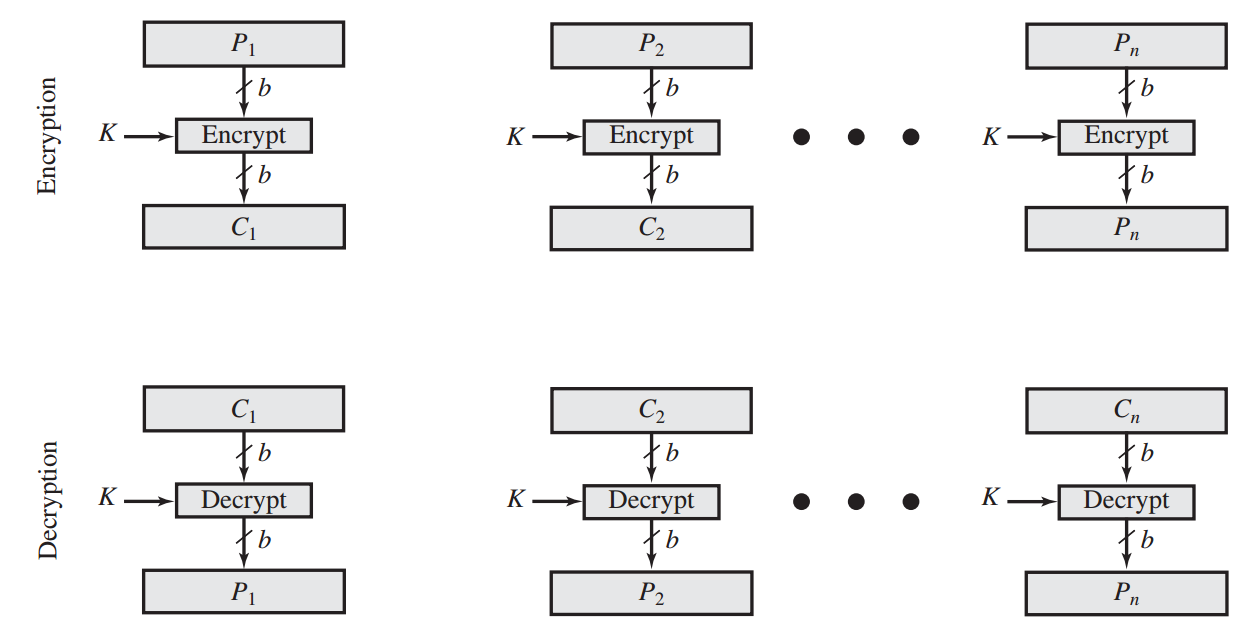
\includegraphics[width=0.7\linewidth]{ECB}
  \end{center}
  \begin{itemize}
  \item<2-> $P_i$ can have a fixed structure
  \item <3-> $P_i$ can repeat
  \item <4-> $C_i$ can be reordered
  \end{itemize}
\end{frame}

\begin{frame}[t]{Finite field algebra}
  \begin{center}
    Properties of $A \oplus B$
  \end{center}
\end{frame}

\begin{frame}[t]{Cipher Block Chaining}
  \begin{center}
    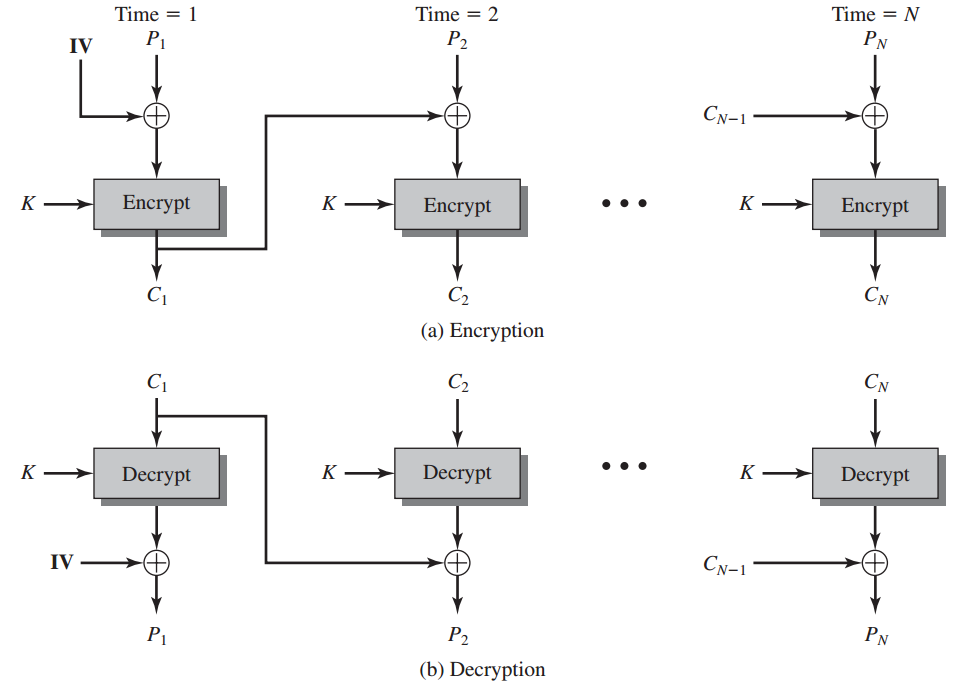
\includegraphics[width=0.7\linewidth]{CBC}
  \end{center}
  \begin{itemize}
  \item<2-> If the received is fooled to use $IV'$ than it decrypts\\
    $P'_1 = IV' \oplus D(K,C_1)$ instead of 
    $P_1 = IV \oplus D(K,C_1)$
  \end{itemize}
\end{frame}

\begin{frame}[t]{Cipher FeedBack}
  \begin{center}
    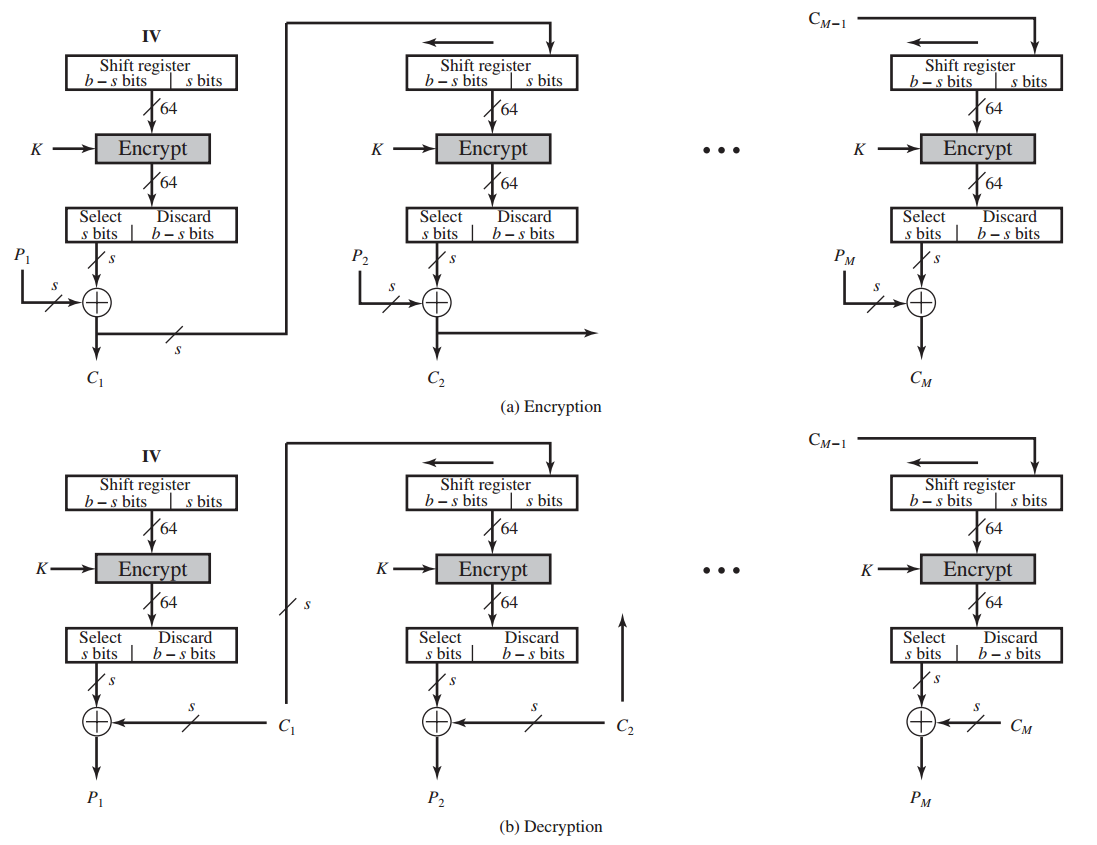
\includegraphics[width=0.7\linewidth]{CFB}
  \end{center}
\end{frame}

\begin{frame}[t]{Counter mode}
  \begin{center}
    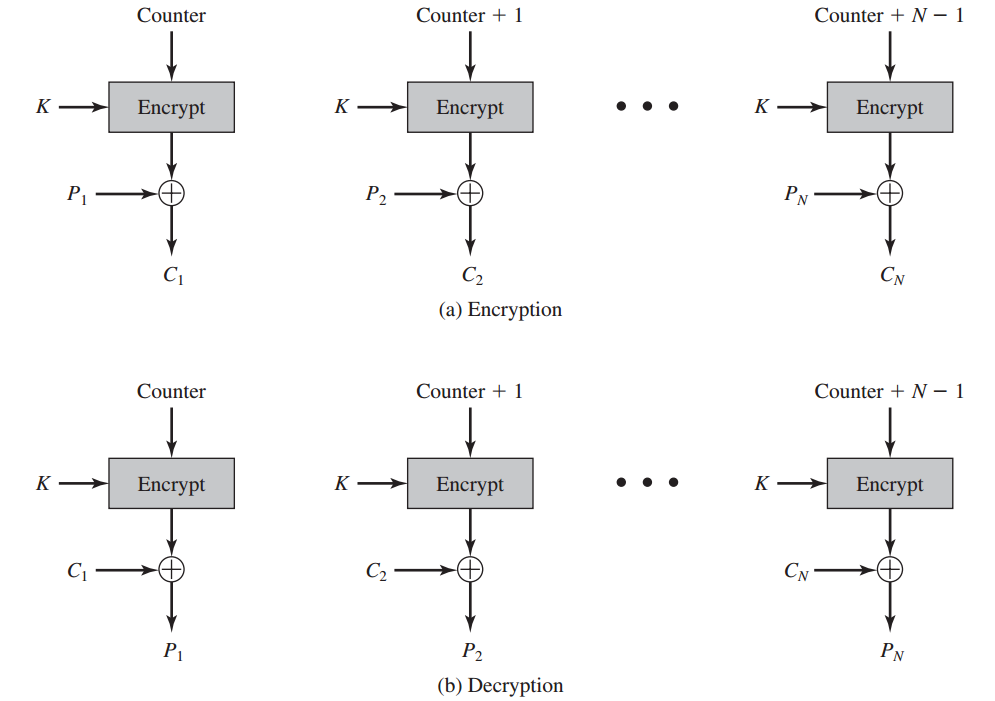
\includegraphics[width=0.7\linewidth]{CTR}
  \end{center}
  \begin{itemize}
  \item<2-> Efficiency, Random access, Provable secure, Requires only
    encryption
  \item<3-> Agreement on the counter
  \end{itemize}
\end{frame}

\begin{frame}{Message authentication}
  \begin{itemize}
\item Symmetric encryption is not enough (e.g. block reordering)
\item Protect integrity
\item Guarantee that the sender is authentic
\item Encryption is expensive
\item Content aware routing
\item Broadcast
  \end{itemize}
\end{frame}

\begin{frame}{Message authentication code}
  \begin{center}
    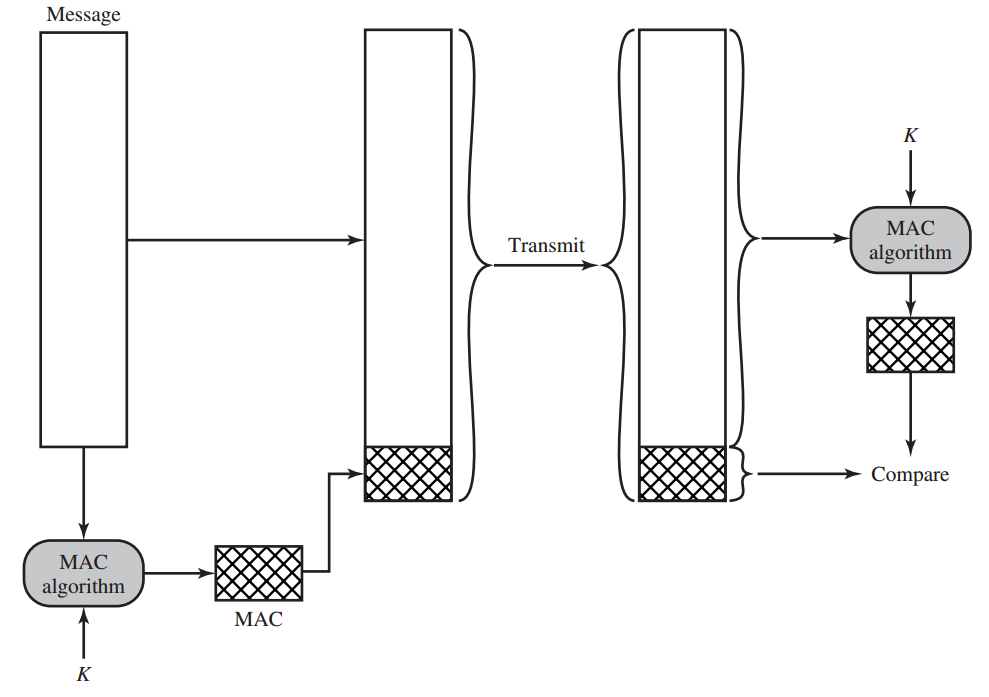
\includegraphics[width=0.6\linewidth]{MAC}
  \end{center}
  \begin{itemize}
\item E.g. last bits of DES(message)
\item Message integrity
\item Sender authenticity
\item With sequence numbers, proper sequence
  \end{itemize}
\end{frame}

\begin{frame}{One way Hash functions}
  \begin{center}
    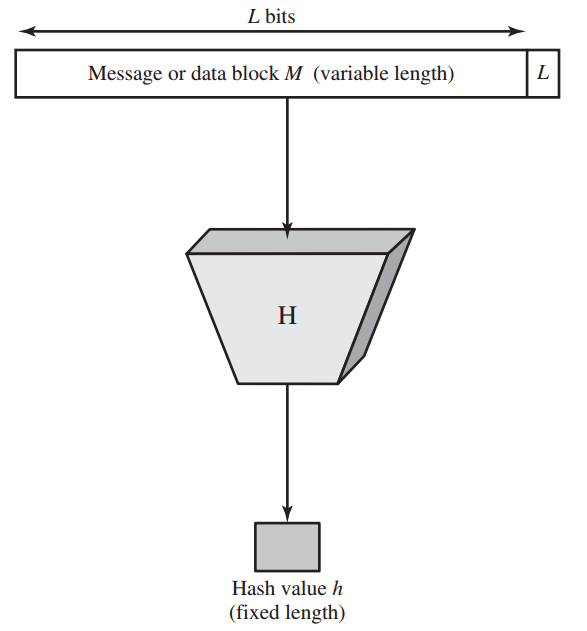
\includegraphics[width=0.5\linewidth]{HASH}
  \end{center}
  \begin{itemize}
\item Encryption is expensive
  \end{itemize}
\end{frame}

\begin{frame}{Authentication via Hash functions}
  \begin{center}
    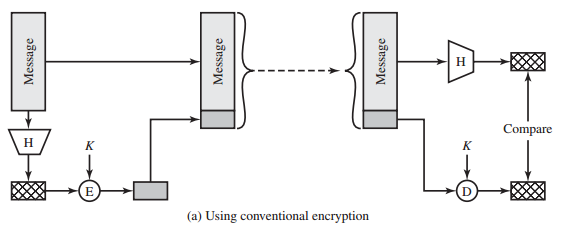
\includegraphics[width=0.7\linewidth]{AuthHASH1}
  \end{center}
\end{frame}
\begin{frame}{Authentication via Hash functions}
  \begin{center}
    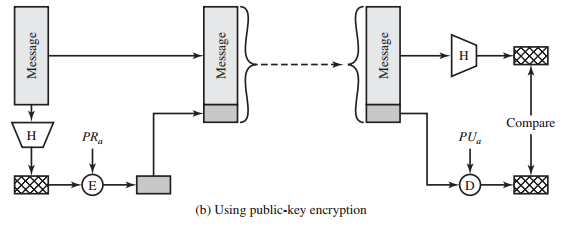
\includegraphics[width=0.7\linewidth]{AuthHASH2}
  \end{center}
\end{frame}
\begin{frame}{Authentication via Hash functions}
  \begin{center}
    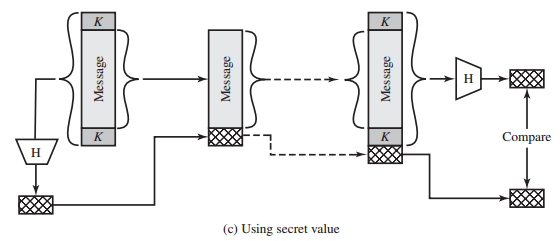
\includegraphics[width=0.7\linewidth]{AuthHASH3}
  \end{center}
\end{frame}

\begin{frame}{Requirements for a secure Hash Function}
  \begin{itemize}
  \item $H$ can be applied to a block of arbitrary size
  \item $H$ produces a fixed length output
  \item $H(x)$ is relatively easy to compute
  \item one-way/preimage resistant:\\
    let $h$ be a code, it is ``infeasible'' to find $x$
    such that $H(x)=h$
  \item weak collision/second preimage resistant:\\
    let $x$ be a block, it is ``infeasible'' to find $y \neq x$
    such that $H(x)=H(y)$
  \item strong  collision resistant:\\
    it is ``infeasible'' to find $(x,y)$ such that $H(x)=H(y)$
  \end{itemize}
\end{frame}

\begin{frame}{Questions?}
  Questions?
\end{frame}

\begin{frame}{Requirements for a secure Hash Function}
  Example
\end{frame}

\begin{frame}{Requirements for a secure Hash Function}
  \begin{itemize}
  \item<1-> What happen if $H(x)$ is difficult to compute?
  \item<2-> What happen if it is not one-way?
  \item<3-> What happen if it is not weak collision resistant?
  \item<4> What happen if it is not strong  collision resistant?
  \end{itemize}
\end{frame}

\begin{frame}{Hash functions}
  \begin{itemize}
  \item To brake weak collision resistant using brute force: $2^{bits}$ attempts
  \item To brake strong collision resistant using brute force: $2^{bits/2}$ attempts
  \item MD5: 128 bits
    \begin{itemize}
      \item 2013 attack on collision resistance in $2^{18}$ attempts: less than a second
    \end{itemize}
  \item SHA-1: 160 bits
    \begin{itemize}
      \item 2011 attack on collision resistance in $2^{60}$
        attempts. no actual collisions are publicly known. 
    \end{itemize}
  \item SHA-2: 224, 256, 384, or 512 bits
  \item Reverse-lookup table: $2^{bits}*(bits/8)$ bytes
  \item Rainbow-tables
  \end{itemize}
\end{frame}

\begin{frame}{Feistel Cipher Structure}
  \begin{center}
    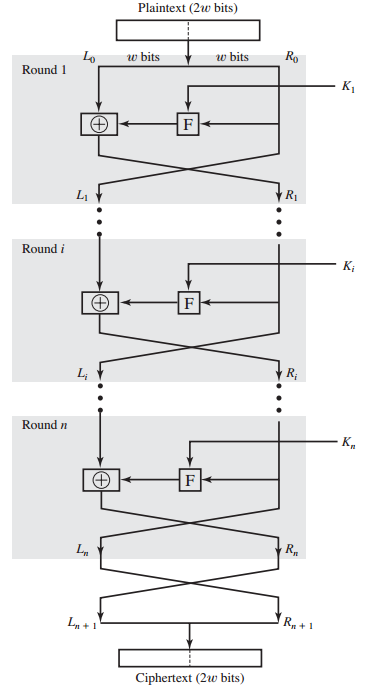
\includegraphics[width=0.35\linewidth]{Feistel}
  \end{center}
\end{frame}

\begin{frame}{Data Encryption Standard (DES)}
  \begin{itemize}
  \item 56 bits key, 64 bits blocks 
  \item Feistel Cipher Structure
  \item 16 rounds, 16 sub-keys derived from the master key
  \item Decryption is basically encryption in reverse order
  \item Triple-$Des$ = $Des(Des^{-1}(Des, K1), K2), K3)$
  \item Triple-$Des^{-1}$ = $Des^{-1}(Des(Des^{-1}, K3), K2), K1)$
  \end{itemize}
\end{frame}

\begin{frame}{Advanced Encryption Standard}
  \begin{itemize}
  \item DES is weak
  \item Triple-Des is expensive
  \item If DES is non-secure then Triple-Des is non-secure
  \end{itemize}
\end{frame}

  \begin{frame}{Advanced Encryption Standard}
  \begin{center}
    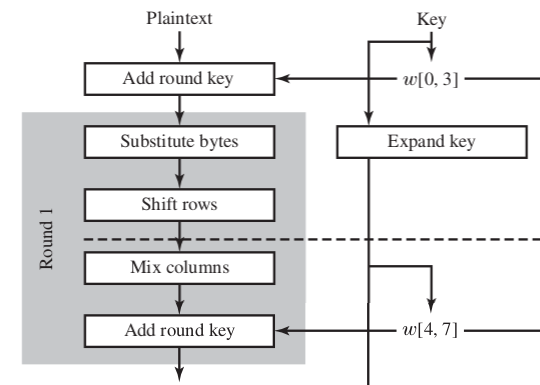
\includegraphics[width=0.50\linewidth]{AES-round}
  \end{center}
\end{frame}

\begin{frame}{Advanced Encryption Standard}
  \begin{center}
    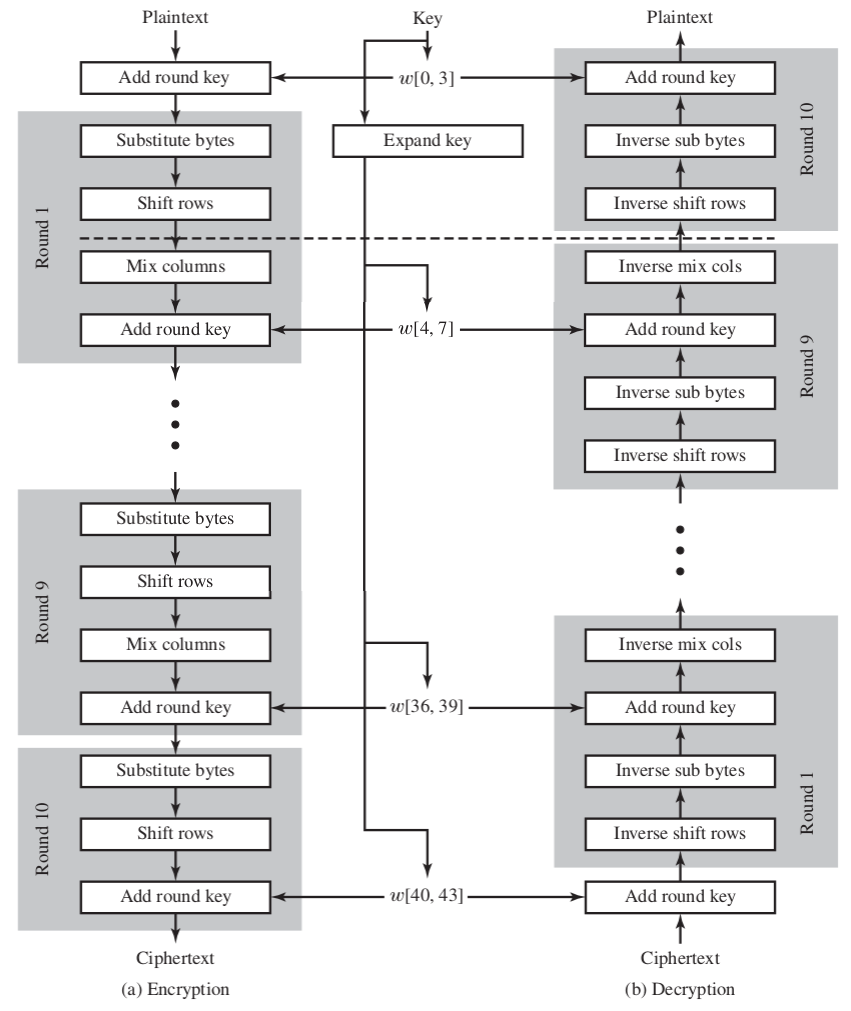
\includegraphics[width=0.50\linewidth]{AES}
  \end{center}
\end{frame}

\begin{frame}{Advanced Encryption Standard}
\begin{columns}[onlytextwidth]
    \begin{column}{0.6\textwidth}
  \begin{center}
    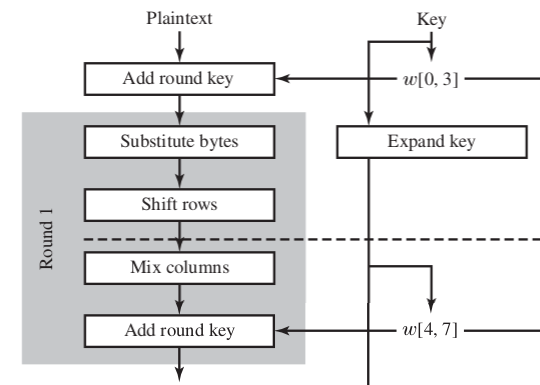
\includegraphics[width=1\linewidth]{AES-round}
  \end{center}
    \end{column}
    \begin{column}{0.4\textwidth}
  \begin{itemize}
  \item Substitute Bytes
  \item Uses a table, referred to as an S-box
  \item Byte-by-byte substitution of the block
  \end{itemize}
    \end{column}
    \end{columns}
\end{frame}

\begin{frame}{Advanced Encryption Standard}
\begin{columns}[onlytextwidth]
    \begin{column}{0.6\textwidth}
  \begin{center}
    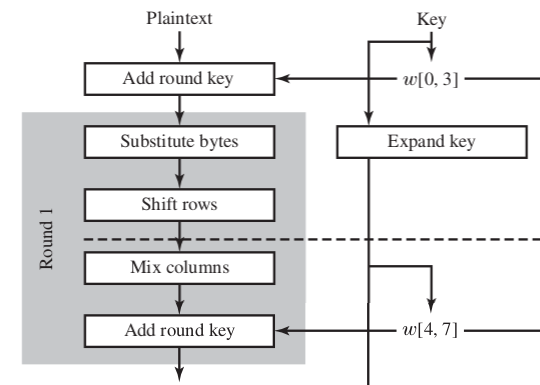
\includegraphics[width=1\linewidth]{AES-round}
  \end{center}
    \end{column}
    \begin{column}{0.4\textwidth}
  \begin{itemize}
  \item ShiftRows
  \item 128bit block seen as matrix of 4x4 bytes
  \end{itemize}
    \end{column}
    \end{columns}
\end{frame}

\begin{frame}{Advanced Encryption Standard}
\begin{columns}[onlytextwidth]
    \begin{column}{0.6\textwidth}
  \begin{center}
    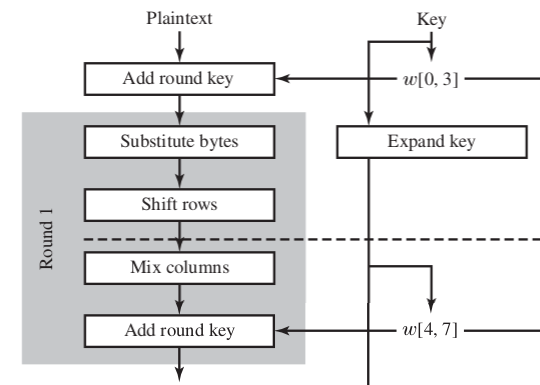
\includegraphics[width=1\linewidth]{AES-round}
  \end{center}
    \end{column}
    \begin{column}{0.4\textwidth}
  \begin{itemize}
  \item Mix Columns
  \item 128bit block seen as matrix of 4x4 bytes
  \item Alters each byte in a column as a function
    of all of the bytes in the column
  \end{itemize}
    \end{column}
    \end{columns}
\end{frame}

\begin{frame}{Advanced Encryption Standard}
\begin{columns}[onlytextwidth]
    \begin{column}{0.6\textwidth}
  \begin{center}
    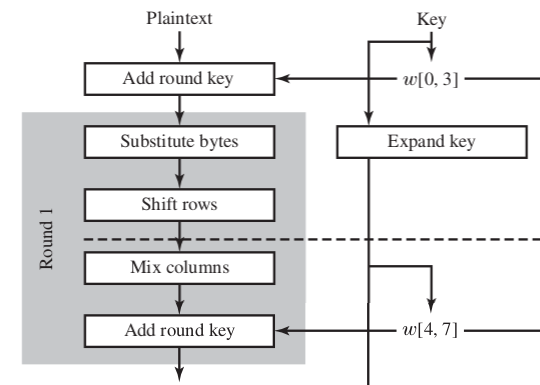
\includegraphics[width=1\linewidth]{AES-round}
  \end{center}
    \end{column}
    \begin{column}{0.4\textwidth}
  \begin{itemize}
  \item Add Round key
  \item Xor with the round key
  \end{itemize}
    \end{column}
    \end{columns}
\end{frame}


\begin{frame}{AES}
  \begin{itemize}
  \item It is not a Feistel structure, process the entire data block in parallel
  \item Each stage is easily reversible
  \item The decryption algorithm makes use of the
    expanded key in reverse order
  \item Only the Add Round Key use of the key. Any other stage,
    is reversible without knowledge of the key
  \end{itemize}
\end{frame}

\begin{frame}{Questions?}
  Questions?
\end{frame}

\end{document}

%%  LocalWords:  decrypt
